\chapter{Planning} \label{plan}

This section will begin to plan the project. The development for this project will be iterative; meaning we will keep evaluating and then attempting to improve the performance. This approach is inspired by the APOD cycle proposed by Nvidia when paralleling code \cite{BradleyNvid}. Of course we are not looking to parallelize code in this, so our cycle is slightly different:\\\\\\

\begin{figure}[H]
\centering
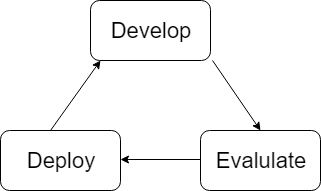
\includegraphics{figures/diagram.png}
\caption{Development Diagram}
\end{figure}

\section{Risk Analysis} \label{risk}

\begin{table}[H]
\centering
\begin{tabular}{|c|m{5cm}|c|c|c|m{5cm}|} 
 \hline
 Rank & Risk & Likelihood & Impact & Exposure & Action \\ [0.5ex] 
 \hline\hline
 
1& Unable to complete all project requirements on time&2&4&6&Weekly meetings with project supervisor. Prioritise different parts of the project \\ 
\hline
2&Problems in understanding affect analysis concepts and literature&2&3&6&Weekly meeting with project supervisor to check progress.  Personal reading on existing literature \\ 
\hline
3&Violating the twitter fair usage policy; I.e returning more tweets then allowed by the API&1&3&3&Ensure we track how many tweets we a processing \\ 
\hline
4&Changes in the twitter api would break existing functionality&2&2&6&Use software design principles to encapsulate access to the twitter API in consideration for potential changes \\ 
\hline
5&Project goes beyond schedule&2&3&6&Use a Gnatt chart to monitor progress and plan effectively \\ 
\hline
6&Problems in understanding the existing solution&1&3&6&Prerequisite action was taken to run the existing solution and understand the code \\ 
\hline
7&Total reliance on twitter streaming API&1&4&3&There are other 3rd patty API's we could use. \\ 
\hline
\end{tabular}

\end{table}

\section{Project Plan} \label{gnatt}


\begin{figure}[H]
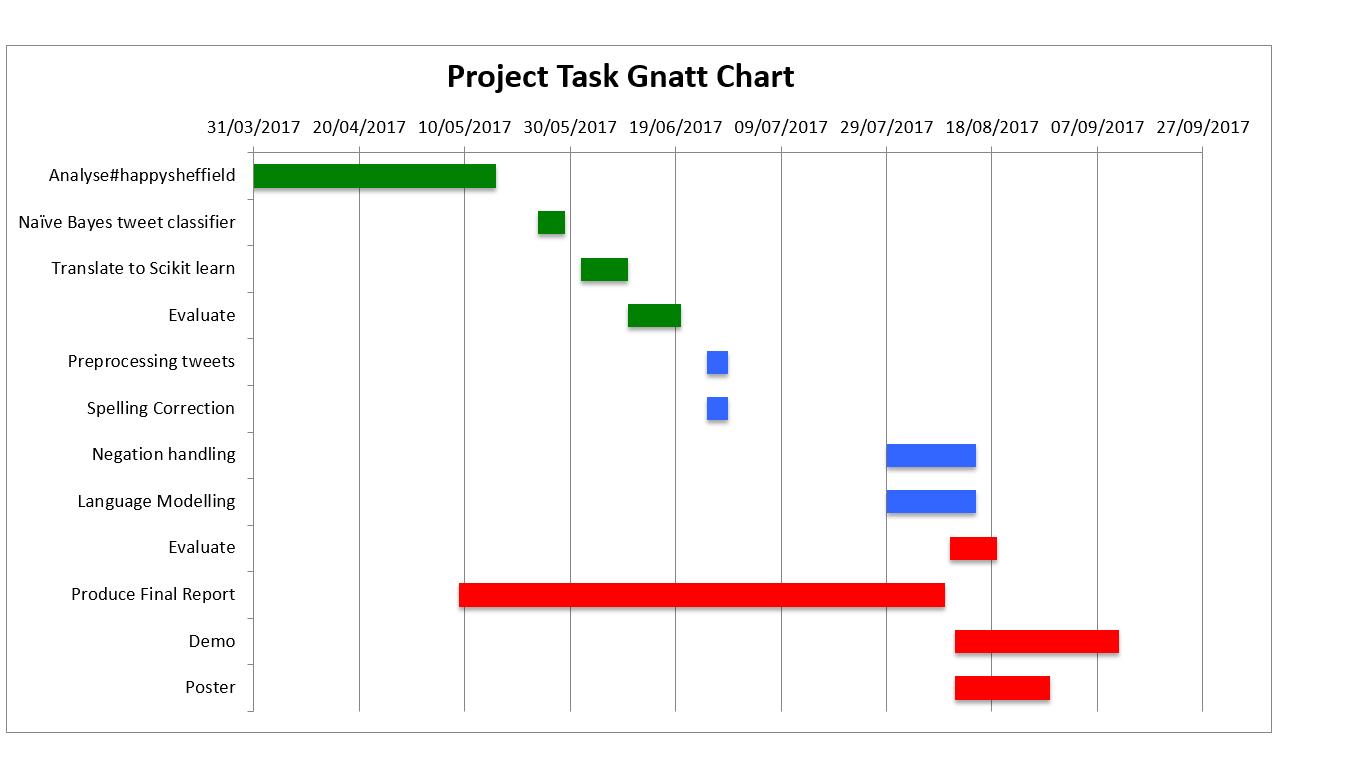
\includegraphics[width=18cm]{images/gnatt.PNG}
\caption{Gnatt Chart}
\end{figure}

\subsection{Task Breakdown}

We will need to produce a methodology describing how we will implement the techniques.

The project will involve an iterative style of development. We will assess the performance of our changes after each iteration. We can break down our tasks as follows:

Work Item 1\\
1.1 Begin Iteration 1\\
1.2 Analyse the \#happysheffield performance \textbf{[Completed]}\\
1.3 Implement a Naive Bayes version of the tweet classification\\
1.4 Use existing ML library \cite{scikit} for a more optimized implementation. \\
1.5 Analyse Results\\

Work Item 2\\
2.1 Begin Iteration 2\\
2.2 Tweak/improve existing implementation\\
\indent{2.2.1 Negation handling}\\
2.3 Analyse Results\\

Work Item 3\\
3.1 Begin Iteration 3\\
3.2 Tweak/improve existing implementation\\
\indent{3.2.1 Spelling Correction}\\
\indent{3.2.2 Language Model Evaluation}\\
3.3 Analyse Results\\

Work Item 4\\
4.1 Produce final report\\

Work Item 5\\
5.1 Produce demo\\
5.2 Produce poster\\



